% Practice Test 09 — Virginia Edition
% Questions: 30 (21 MC + 9 SA)
% Generated by scripts/generate_practice_tests.py

\begin{practiceQuestion}{1-4-q14}{mc}
\begin{questionText}
A proportional relationship has the equation $y = \frac{2}{5}x$. What is $y$ when $x = 20$?
\end{questionText}
\choiceA{$4$}
\choiceB{$8$}
\choiceC{$10$}
\choiceD{$50$}
\correctAnswer{B}
\explanation{$y = \frac{2}{5} \times 20 = \frac{40}{5} = 8$.}
\end{practiceQuestion}

\begin{practiceQuestion}{2-1-q10}{mc}
\begin{questionText}
What is $8\%$ of $250$?
\end{questionText}
\choiceA{$2$}
\choiceB{$16$}
\choiceC{$20$}
\choiceD{$32$}
\correctAnswer{C}
\explanation{$8\% = 0.08$. Multiply: $0.08 \times 250 = 20$.}
\end{practiceQuestion}

\begin{practiceQuestion}{2-2-q23}{sa}
\begin{questionText}
In a survey, $51$ out of $300$ people chose vanilla ice cream. What percent chose vanilla?
\end{questionText}
\correctAnswer{$17\%$}
\explanation{$\frac{51}{300} = \frac{p}{100}$. Cross-multiply: $300p = 5100$. Divide: $p = 17\%$.}
\end{practiceQuestion}

\begin{practiceQuestion}{2-3-q02}{mc}
\begin{questionText}
A population grew from $5{,}000$ to $5{,}750$. What is the percent increase?
\end{questionText}
\choiceA{$12\%$}
\choiceB{$13\%$}
\choiceC{$15\%$}
\choiceD{$17.5\%$}
\correctAnswer{C}
\explanation{Change: $5{,}750 - 5{,}000 = 750$. Percent change: $750 \div 5{,}000 = 0.15 = 15\%$.}
\end{practiceQuestion}

\begin{practiceQuestion}{2-7-q15}{mc}
\begin{questionText}
A chemist expected to collect $75$ mL of solution but collected $80$ mL. What is the percent error (rounded to the nearest tenth)?
\end{questionText}
\choiceA{$5\%$}
\choiceB{$6.3\%$}
\choiceC{$6.7\%$}
\choiceD{$7.5\%$}
\correctAnswer{B}
\explanation{$\frac{|75 - 80|}{80} \times 100 = \frac{5}{80} \times 100 = 6.25 \approx 6.3\%$.}
\end{practiceQuestion}

\begin{practiceQuestion}{3-2-q06}{mc}
\begin{questionText}
The temperature is $-4°$C at dawn. By noon it rises $10°$C. What is the noon temperature?
\end{questionText}
\choiceA{$-14°$C}
\choiceB{$14°$C}
\choiceC{$-6°$C}
\choiceD{$6°$C}
\correctAnswer{D}
\explanation{$(-4) + 10 = 6$. Different signs: $10 - 4 = 6$. The larger absolute value is positive.}
\end{practiceQuestion}

\begin{practiceQuestion}{3-3-q21}{sa}
\begin{questionText}
Find the distance between $-11$ and $-3$ on a number line.
\end{questionText}
\correctAnswer{$8$ units}
\explanation{Distance $= |{-11} - (-3)| = |{-11} + 3| = |{-8}| = 8$ units.}
\end{practiceQuestion}

\begin{practiceQuestion}{3-4-q07}{mc}
\begin{questionText}
What is $-\dfrac{3}{5} + \dfrac{3}{5}$?
\end{questionText}
\choiceA{$\dfrac{6}{5}$}
\choiceB{$-\dfrac{6}{5}$}
\choiceC{$0$}
\choiceD{$\dfrac{6}{10}$}
\correctAnswer{C}
\explanation{A number plus its opposite equals $0$: $-\frac{3}{5} + \frac{3}{5} = 0$.}
\end{practiceQuestion}

\begin{practiceQuestion}{4-3-q19}{sa}
\begin{questionText}
Expand $-6(2m - 5)$.
\end{questionText}
\correctAnswer{$-12m + 30$}
\explanation{$-6 \times 2m = -12m$ and $-6 \times (-5) = +30$. Result: $-12m + 30$.}
\end{practiceQuestion}

\begin{practiceQuestion}{4-4-q28}{gmc}
\begin{questionText}
The rectangle below has the given area. Which pair of dimensions is correct?

\begin{center}
\begin{tikzpicture}[scale=0.7]
  \draw[thick, fill=funBlue!10] (0,0) rectangle (6,2.5);
  \node at (3,1.25) {Area $= 10x + 35$};
  \node[left] at (0,1.25) {?};
  \node[below] at (3,0) {?};
\end{tikzpicture}
\end{center}
\end{questionText}
\choiceA{Width $= 5$, Length $= 2x + 7$}
\choiceB{Width $= 10$, Length $= x + 35$}
\choiceC{Width $= 5$, Length $= 2x + 35$}
\choiceD{Width $= 2$, Length $= 5x + 35$}
\correctAnswer{A}
\explanation{Factor: $10x + 35 = 5(2x + 7)$. So the width is $5$ and the length is $2x + 7$.}
\end{practiceQuestion}

\begin{practiceQuestion}{5-4-q26}{gmc}
\begin{questionText}
The table shows input and output values for a function. What is the rule?

\begin{center}
\begin{tabular}{|c|c|}
\hline
\textbf{Input ($x$)} & \textbf{Output ($y$)} \\
\hline
$2$ & $2.5$ \\
\hline
$4$ & $3.5$ \\
\hline
$6$ & $4.5$ \\
\hline
$10$ & $6.5$ \\
\hline
\end{tabular}
\end{center}
\end{questionText}
\choiceA{$y = 0.5x + 1.5$}
\choiceB{$y = x - 0.5$}
\choiceC{$y = 0.25x + 2$}
\choiceD{$y = 2x - 1.5$}
\correctAnswer{A}
\explanation{From $x = 2$ to $x = 4$, $y$ increases by $1$ while $x$ increases by $2$, so rate $= 0.5$. When $x = 2$: $0.5(2) + 1.5 = 2.5$ \checkmark.}
\end{practiceQuestion}

\begin{practiceQuestion}{5-5-q03}{mc}
\begin{questionText}
Which inequality represents ``at most $15$''?
\end{questionText}
\choiceA{$x > 15$}
\choiceB{$x < 15$}
\choiceC{$x \geq 15$}
\choiceD{$x \leq 15$}
\correctAnswer{D}
\explanation{``At most'' means $15$ or less, which is $x \leq 15$.}
\end{practiceQuestion}

\begin{practiceQuestion}{5-6-q10}{mc}
\begin{questionText}
Solve $5 - x > 8$ and describe the graph.
\end{questionText}
\choiceA{Open circle at $3$, shade right}
\choiceB{Open circle at $-3$, shade left}
\choiceC{Closed circle at $-3$, shade left}
\choiceD{Open circle at $-3$, shade right}
\correctAnswer{B}
\explanation{Subtract $5$: $-x > 3$. Multiply by $-1$ and flip: $x < -3$. Open circle at $-3$, shade left.}
\end{practiceQuestion}

\begin{practiceQuestion}{6-1-q28}{gmc}
\begin{questionText}
The scale drawing below shows a rectangular garden with scale $1$ cm $= 3$ m. Which statement is correct about the actual garden?

\begin{center}
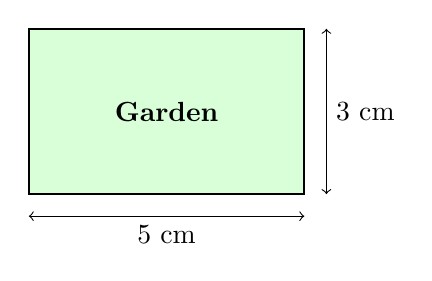
\begin{tikzpicture}[scale=0.7]
  \draw[thick,fill=green!15] (0,0) rectangle (5,3);
  \draw[<->] (0,-0.4) -- (5,-0.4);
  \node[below] at (2.5,-0.4) {$5$ cm};
  \draw[<->] (5.4,0) -- (5.4,3);
  \node[right] at (5.4,1.5) {$3$ cm};
  \node at (2.5,1.5) {\textbf{Garden}};
\end{tikzpicture}
\end{center}
\end{questionText}
\choiceA{The actual garden has an area of $15$ m$^2$}
\choiceB{The actual garden has a perimeter of $48$ m}
\choiceC{The actual garden has an area of $135$ m$^2$}
\choiceD{The actual garden has a perimeter of $16$ m}
\correctAnswer{C}
\explanation{Actual dimensions: $5 \times 3 = 15$ m and $3 \times 3 = 9$ m. Area: $15 \times 9 = 135$ m$^2$. Perimeter: $2(15 + 9) = 48$ m. Both B and C look plausible, but the area of $135$ m$^2$ matches choice C.}
\end{practiceQuestion}

\begin{practiceQuestion}{6-2-q03}{mc}
\begin{questionText}
A model uses scale $1:100$. You need to redraw it at scale $1:50$. A wall that is $4$ cm on the original model becomes how long?
\end{questionText}
\choiceA{$2$ cm}
\choiceB{$4$ cm}
\choiceC{$8$ cm}
\choiceD{$200$ cm}
\correctAnswer{C}
\explanation{Scale ratio: $\frac{100}{50} = 2$. New length: $4 \times 2 = 8$ cm.}
\end{practiceQuestion}

\begin{practiceQuestion}{6-5-q05}{mc}
\begin{questionText}
You slice a rectangular pyramid with a cut parallel to the base, halfway up. What shape is the cross-section?
\end{questionText}
\choiceA{A triangle}
\choiceB{A smaller rectangle}
\choiceC{A circle}
\choiceD{A pentagon}
\correctAnswer{B}
\explanation{A horizontal cut parallel to the base of a rectangular pyramid gives a rectangle. It is smaller than the base because the pyramid narrows toward the apex.}
\end{practiceQuestion}

\begin{practiceQuestion}{6-6-q02}{mc}
\begin{questionText}
Two angles are complementary. One angle is $27°$. What is the other angle?
\end{questionText}
\choiceA{$53°$}
\choiceB{$63°$}
\choiceC{$73°$}
\choiceD{$153°$}
\correctAnswer{B}
\explanation{Complementary angles sum to $90°$. $90° - 27° = 63°$.}
\end{practiceQuestion}

\begin{practiceQuestion}{6-7-q22}{sa}
\begin{questionText}
A triangle has vertices $A(2, 1)$, $B(6, 1)$, and $C(6, 4)$. Reflect the triangle over the $y$-axis. List the new vertices.
\end{questionText}
\correctAnswer{$A'(-2, 1)$, $B'(-6, 1)$, $C'(-6, 4)$}
\explanation{Over the $y$-axis: negate $x$, keep $y$. $(2,1) \to (-2,1)$, $(6,1) \to (-6,1)$, $(6,4) \to (-6,4)$.}
\end{practiceQuestion}

\begin{practiceQuestion}{6-8-q29}{gsa}
\begin{questionText}
The two triangles below are similar. Find the missing side lengths $a$ and $b$.

\begin{center}
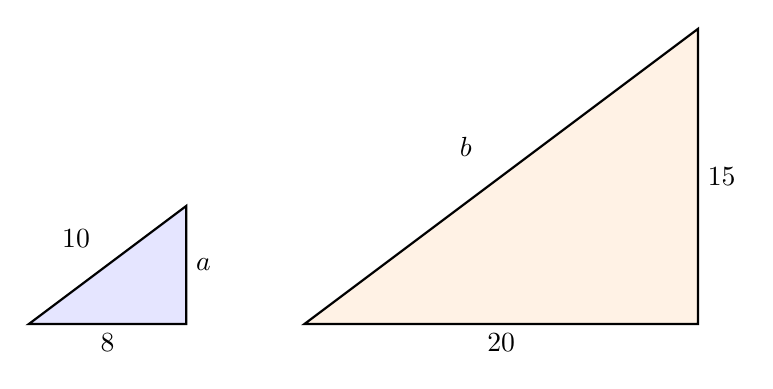
\begin{tikzpicture}[scale=0.5]
  % Small triangle
  \draw[thick,fill=blue!10] (0,0) -- (4,0) -- (4,3) -- cycle;
  \node[below] at (2,0) {$8$};
  \node[right] at (4,1.5) {$a$};
  \node[above left] at (1.8,1.7) {$10$};
  % Large triangle
  \draw[thick,fill=orange!10] (7,0) -- (17,0) -- (17,7.5) -- cycle;
  \node[below] at (12,0) {$20$};
  \node[right] at (17,3.75) {$15$};
  \node[above left] at (11.5,4) {$b$};
\end{tikzpicture}
\end{center}
\end{questionText}
\correctAnswer{$a = 6$, $b = 25$}
\explanation{Scale factor from small to large: $\frac{20}{8} = 2.5$. $a$: from large to small on the right side $= 15 \div 2.5 = 6$. $b$: from small to large on the hypotenuse $= 10 \times 2.5 = 25$.}
\end{practiceQuestion}

\begin{practiceQuestion}{7-4-q12}{mc}
\begin{questionText}
A square has sides of $10$ m. A quarter circle with radius $10$ m is removed from one corner. What is the area of the remaining figure? Use $\pi \approx 3.14$.
\end{questionText}
\choiceA{$21.5$ m$^2$}
\choiceB{$50$ m$^2$}
\choiceC{$78.5$ m$^2$}
\choiceD{$100$ m$^2$}
\correctAnswer{A}
\explanation{Square: $100$ m$^2$. Quarter circle: $\frac{1}{4} \times 3.14 \times 100 = 78.5$ m$^2$. Remaining: $100 - 78.5 = 21.5$ m$^2$.}
\end{practiceQuestion}

\begin{practiceQuestion}{7-5-q03}{mc}
\begin{questionText}
A rectangular box is $10$ in by $6$ in by $4$ in. What is the total surface area?
\end{questionText}
\choiceA{$120$ in$^2$}
\choiceB{$240$ in$^2$}
\choiceC{$248$ in$^2$}
\choiceD{$148$ in$^2$}
\correctAnswer{C}
\explanation{$SA = 2(10 \times 6) + 2(10 \times 4) + 2(6 \times 4) = 120 + 80 + 48 = 248$ in$^2$.}
\end{practiceQuestion}

\begin{practiceQuestion}{7-6-q23}{sa}
\begin{questionText}
A rectangular prism has a volume of $360$ cm$^3$. Its length is $12$ cm and its height is $5$ cm. What is its width?
\end{questionText}
\correctAnswer{$6$ cm}
\explanation{$360 = 12 \times w \times 5 = 60w$. $w = 360 \div 60 = 6$ cm.}
\end{practiceQuestion}

\begin{practiceQuestion}{7-7-q24}{sa}
\begin{questionText}
Find the surface area of a cylinder with radius $7$ cm and height $10$ cm. Use $\pi \approx \frac{22}{7}$.
\end{questionText}
\correctAnswer{$748$ cm$^2$}
\explanation{$SA = 2\pi r^2 + 2\pi rh = 2 \times \frac{22}{7} \times 49 + 2 \times \frac{22}{7} \times 7 \times 10 = 308 + 440 = 748$ cm$^2$.}
\end{practiceQuestion}

\begin{practiceQuestion}{8-1-q19}{sa}
\begin{questionText}
A random sample of $80$ out of $2{,}000$ students found that $20$ students ride the bus. Predict how many students in the school ride the bus.
\end{questionText}
\correctAnswer{$500$}
\explanation{$\frac{20}{80} = 25\%$. Then $25\%$ of $2{,}000 = 500$.}
\end{practiceQuestion}

\begin{practiceQuestion}{8-3-q04}{mc}
\begin{questionText}
Group X has a median of $50$ and a range of $10$. Group Y has a median of $50$ and a range of $30$. Which statement is true?
\end{questionText}
\choiceA{Group X has more data values}
\choiceB{Group Y has a higher center}
\choiceC{Group Y is more spread out than Group X}
\choiceD{The groups are identical}
\correctAnswer{C}
\explanation{Both have the same median, but Group Y's larger range means its data is more spread out.}
\end{practiceQuestion}

\begin{practiceQuestion}{8-4-q01}{mc}
\begin{questionText}
Data set A: $10, 12, 14, 16, 18$. What is the mean?
\end{questionText}
\choiceA{$12$}
\choiceB{$14$}
\choiceC{$16$}
\choiceD{$70$}
\correctAnswer{B}
\explanation{$\frac{10+12+14+16+18}{5} = \frac{70}{5} = 14$.}
\end{practiceQuestion}

\begin{practiceQuestion}{8-5-q07}{mc}
\begin{questionText}
What is the range of this data set shown in the stem-and-leaf plot?

\begin{center}
\begin{tabular}{r|l}
\textbf{Stem} & \textbf{Leaf} \\
\hline
$2$ & $3\;\;7$ \\
$3$ & $0\;\;4\;\;8$ \\
$4$ & $1\;\;5\;\;5\;\;9$ \\
$5$ & $2$
\end{tabular}
\end{center}
\end{questionText}
\choiceA{$23$}
\choiceB{$29$}
\choiceC{$30$}
\choiceD{$52$}
\correctAnswer{B}
\explanation{Smallest value: $23$. Largest value: $52$. Range $= 52 - 23 = 29$.}
\end{practiceQuestion}

\begin{practiceQuestion}{9-3-q25}{sa}
\begin{questionText}
A spinner is spun $40$ times. Green appears $10$ times, blue appears $18$ times, and yellow appears $12$ times. What is the experimental probability of landing on blue or yellow? Write your answer as a decimal.
\end{questionText}
\correctAnswer{$0.75$}
\explanation{Blue $+$ Yellow $= 18 + 12 = 30$. $P = \frac{30}{40} = 0.75$.}
\end{practiceQuestion}

\begin{practiceQuestion}{9-6-q14}{mc}
\begin{questionText}
A bag has $4$ green and $6$ yellow marbles. You pick one marble without replacement and then pick another. What is the probability that the first is green and the second is yellow?
\end{questionText}
\choiceA{$\frac{24}{100}$}
\choiceB{$\frac{24}{90}$}
\choiceC{$\frac{4}{15}$}
\choiceD{$\frac{6}{10}$}
\correctAnswer{C}
\explanation{$P(\text{green first}) = \frac{4}{10}$. After removing a green, $P(\text{yellow second}) = \frac{6}{9}$. $P = \frac{4}{10} \times \frac{6}{9} = \frac{24}{90} = \frac{4}{15}$.}
\end{practiceQuestion}

\begin{practiceQuestion}{9-7-q06}{mc}
\begin{questionText}
Why are simulations useful?
\end{questionText}
\choiceA{They always give exact answers}
\choiceB{They can estimate probabilities when real experiments are too difficult or impractical}
\choiceC{They replace all mathematical calculations}
\choiceD{They only work for coin flips}
\correctAnswer{B}
\explanation{Simulations estimate probabilities for complex events that are hard to compute directly or where real experiments are impractical.}
\end{practiceQuestion}
